\chapter{Capacidades del prototipo}
\label{chap:capacidades-prototipo}

\section{Cómo leer este capítulo}

% CROSS_REFERENCE_MAPPING_REQUIRED
Este capítulo describe qué hace el prototipo, capacidad por capacidad. Cada sección responde cuatro preguntas en el mismo orden: qué hace la capacidad, cómo funciona, qué evidencia la respalda y qué límites tiene. La decisión de organizarlo así, y no por la secuencia en que cada componente se construyó, responde a que el lector necesita saber de qué es capaz el sistema antes que cuándo se implementó cada parte. La evolución técnica del desarrollo se documenta en el Anexo F.

Las capacidades se presentan en el orden del recorrido del usuario. El estudio ingresa al sistema, se prepara, se segmenta en ambos planos, se derivan mediciones que se asocian a un nivel anatómico, el resultado se visualiza y se navega, el profesional lo revisa y el conjunto se persiste con su trazabilidad. Las dos últimas secciones reúnen las capacidades desarrolladas que no se exponen en el producto y el estado consolidado de todas ellas.

% CROSS_REFERENCE_MAPPING_REQUIRED
Una advertencia de lectura vale para todo el capítulo: capacidad implementada no significa capacidad validada clínicamente. El prototipo produce salidas técnicas verificables contra anotaciones de referencia. Su utilidad clínica no fue evaluada y queda declarada como fuera del alcance en el Capítulo 5.

\section{Ingesta y preparación del estudio}

Qué hace. Recibe un estudio de resonancia magnética lumbar completo, identifica las series que contiene, las clasifica por plano y ponderación, y las prepara para el procesamiento.

Cómo funciona. La vía principal es un estudio en formato DICOM empaquetado, del que el sistema extrae las series y determina cuáles son compatibles con los modelos disponibles. El usuario no selecciona imágenes de a una: la cantidad de cortes se obtiene del propio volumen. Se conserva compatibilidad con otros formatos, empleados como fixtures de prueba y en flujos de investigación.

{\small
\setlength{\LTleft}{0pt}
\setlength{\LTright}{0pt}
\setlength{\tabcolsep}{3pt}
\renewcommand{\arraystretch}{1.18}
\begin{longtable}{>{\raggedright\arraybackslash}p{0.18\textwidth} >{\raggedright\arraybackslash}p{0.38\textwidth} >{\raggedright\arraybackslash}p{0.38\textwidth}}
\caption{Formatos admitidos y uso previsto.}\label{tab:cap-formatos-ingesta}\\
\hline
\textbf{Formato} & \textbf{Uso en el proyecto} & \textbf{Metadata aprovechada} \\
\hline
\endfirsthead
\hline
\textbf{Formato} & \textbf{Uso en el proyecto} & \textbf{Metadata aprovechada} \\
\hline
\endhead
\hline
\endfoot
DICOM & Vía principal de ingesta; estudio completo con sus series registradas & Espaciado de píxel, posición y orientación de la imagen, y demás metadata de serie e instancia \\
MHA y MHD & Compatibilidad técnica, fixtures y flujos de investigación & Dimensiones, espaciado, origen y dirección cuando están disponibles \\
NPY & Pruebas automatizadas y volúmenes controlados & Dimensiones y eje de selección \\
PNG, JPG y otros formatos de imagen & Pruebas mínimas y entradas bidimensionales simples & Sin geometría física confiable \\
\hline
\end{longtable}
}

La preparación normaliza la intensidad recortando por los percentiles 1 y 99 y escalándola al intervalo unitario, y redimensiona la imagen a la dimensión que el modelo espera. Ese redimensionado obliga a una corrección que resulta determinante para las mediciones posteriores: el sistema mantiene tres representaciones geométricas simultáneas, la grilla nativa de la imagen, la grilla del modelo y el espacio del paciente en milímetros, y ajusta el espaciado al pasar de la segunda a la tercera. La corrección se aplica sobre el espaciado y no sobre la medición, porque el error no reside en el recuento de píxeles sino en cuánto mide cada píxel de esa grilla. Sin ella, un corte redimensionado devolvía valores un tercio menores que los reales y áreas afectadas en mayor proporción, dado que el factor interviene al cuadrado.

Antes de ejecutar, el sistema valida el formato y los límites aceptados. La ausencia del plano axial no invalida una corrida sagital.

\begin{figure}[htbp]
\centering
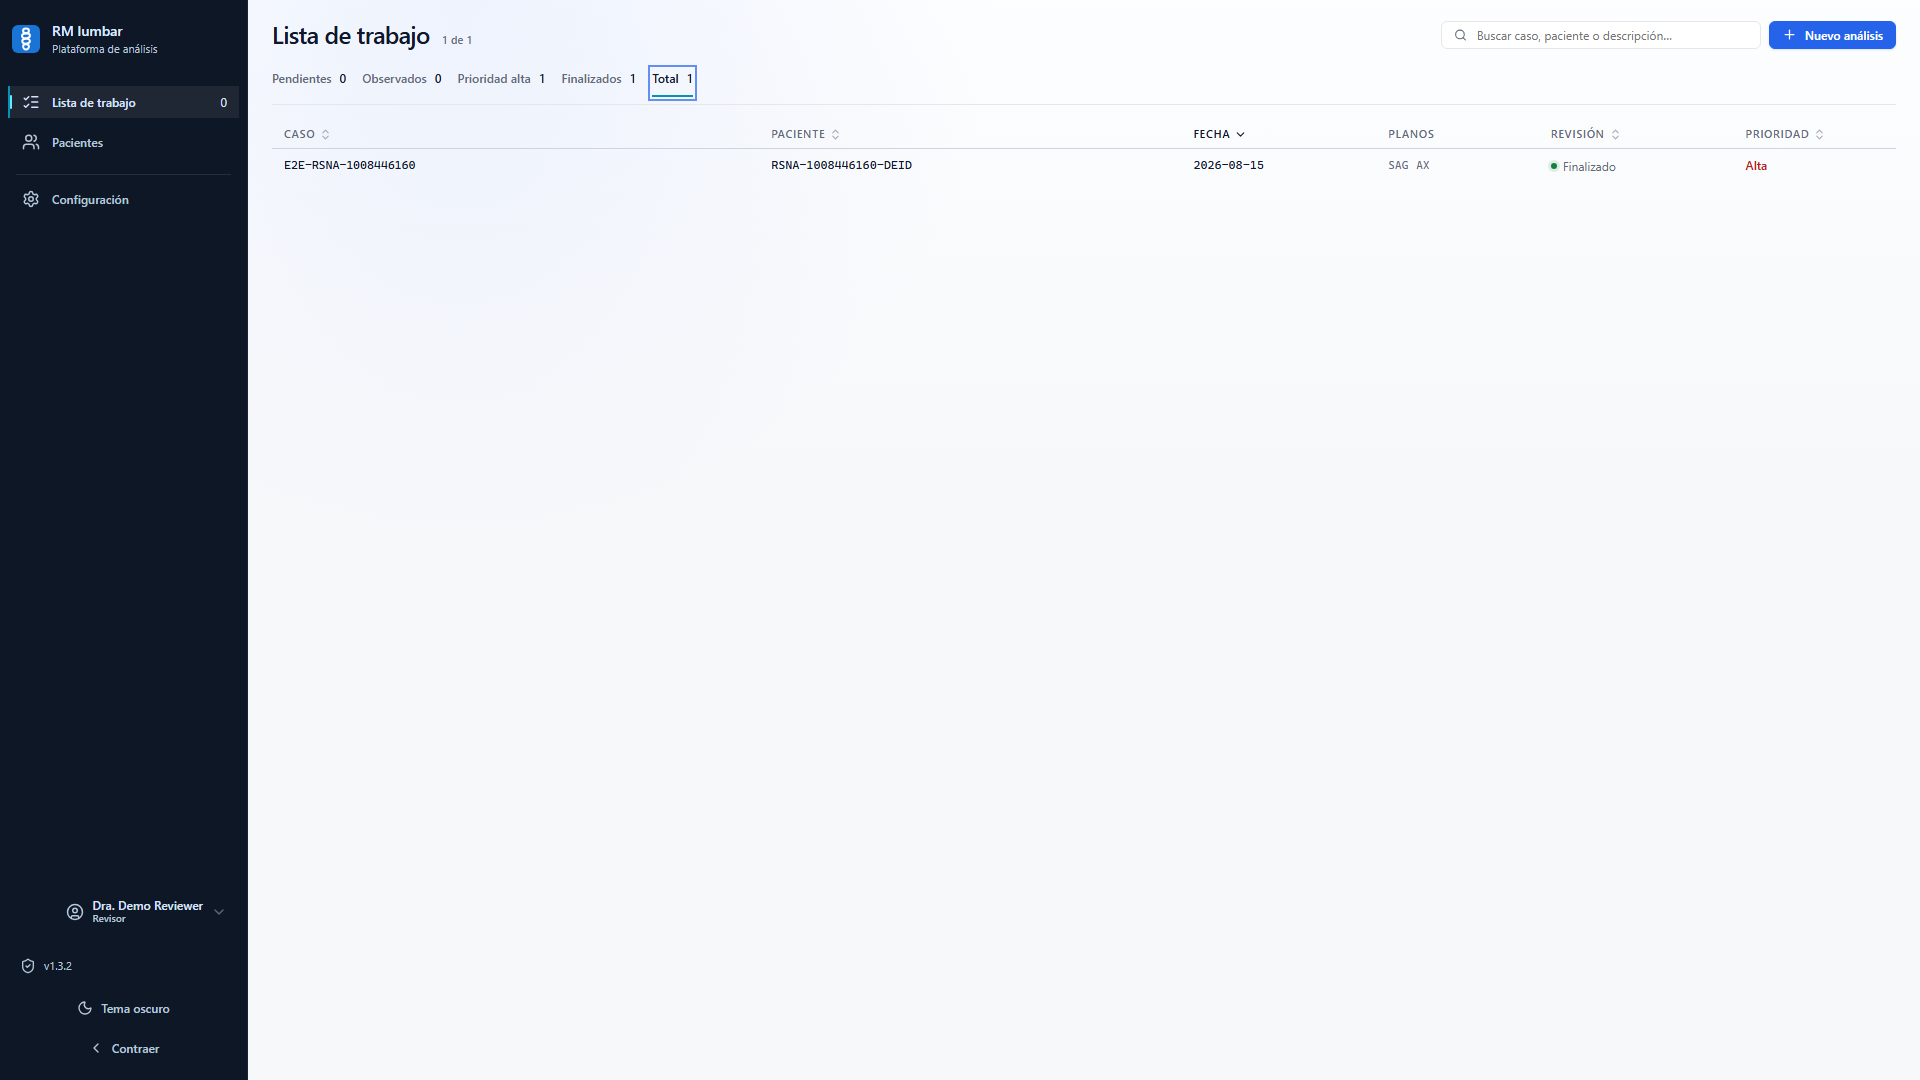
\includegraphics[width=\textwidth]{images/product_screenshots/fig_11_01_acceso_worklist.png}
\caption{Acceso con estado de cuenta pendiente de aprobación y worklist de estudios. Fuente: elaboración propia.}
\label{fig:cap11-acceso-worklist}
\end{figure}

\begin{figure}[htbp]
\centering
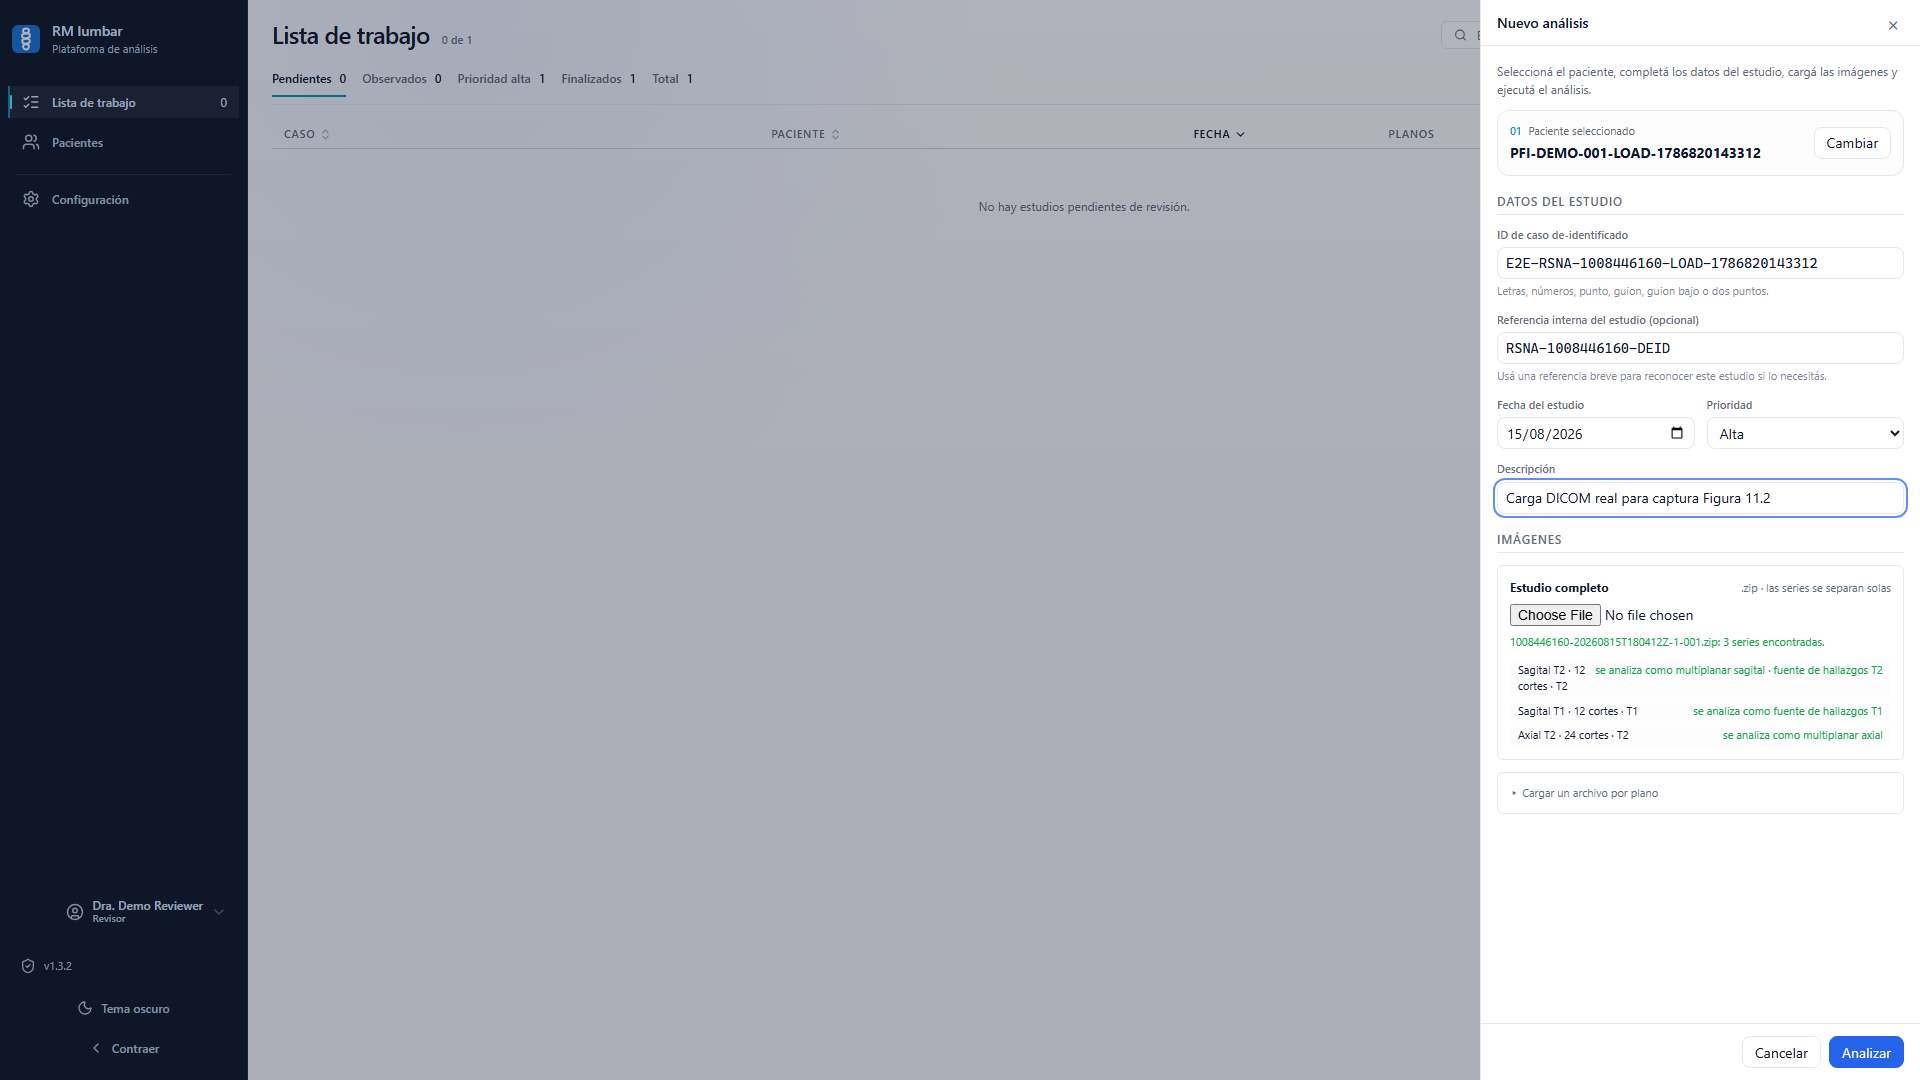
\includegraphics[width=\textwidth]{images/product_screenshots/fig_11_02_carga_estudio_dicom.png}
\caption{Carga de un estudio DICOM con sus series identificadas y clasificadas. Fuente: elaboración propia.}
\label{fig:cap11-carga-estudio-dicom}
\end{figure}
Qué evidencia lo respalda. Pruebas automatizadas de lectura de volúmenes, de preprocesamiento y de selección de corte, y regresión sobre fixtures de-identificados. El acceso requiere autenticación y una cuenta nueva permanece pendiente de aprobación hasta que un administrador la habilite.

Qué límites tiene. Cuando la fuente no aporta espaciado válido, las mediciones derivadas se expresan en píxeles y la unidad lo declara: el sistema no infiere geometría física ausente. Las series y modalidades no soportadas quedan disponibles como imagen base e informan que no poseen inferencia automática.

\section{Segmentación sagital}

Qué hace. Delimita, sobre cortes sagitales, tres tipos de estructura: cuerpos vertebrales, canal espinal y discos intervertebrales.

Cómo funciona. Una red convolucional bidimensional de tipo U-Net, entrenada sobre el conjunto SPIDER, que produce una máscara de cuatro clases: fondo, vértebras, canal y discos. Las vértebras y los discos se segmentan como clase agrupada, no como instancias individuales; la separación por espacio discal se resuelve en el postprocesamiento, según se describe en la sección~\ref{sec:cap-asignacion-nivel-anatomico}. El procesamiento se aplica a la serie completa y no únicamente al corte de referencia.

Cada corrida resuelve el artifact correspondiente al plano solicitado, verifica que su manifest y su arquitectura sean compatibles y ejecuta la inferencia. La carga es estricta: si los nombres de capa del artifact no coinciden con los de la arquitectura declarada, la carga falla de forma explícita en lugar de completar los pesos faltantes.

\begin{figure}[htbp]
\centering
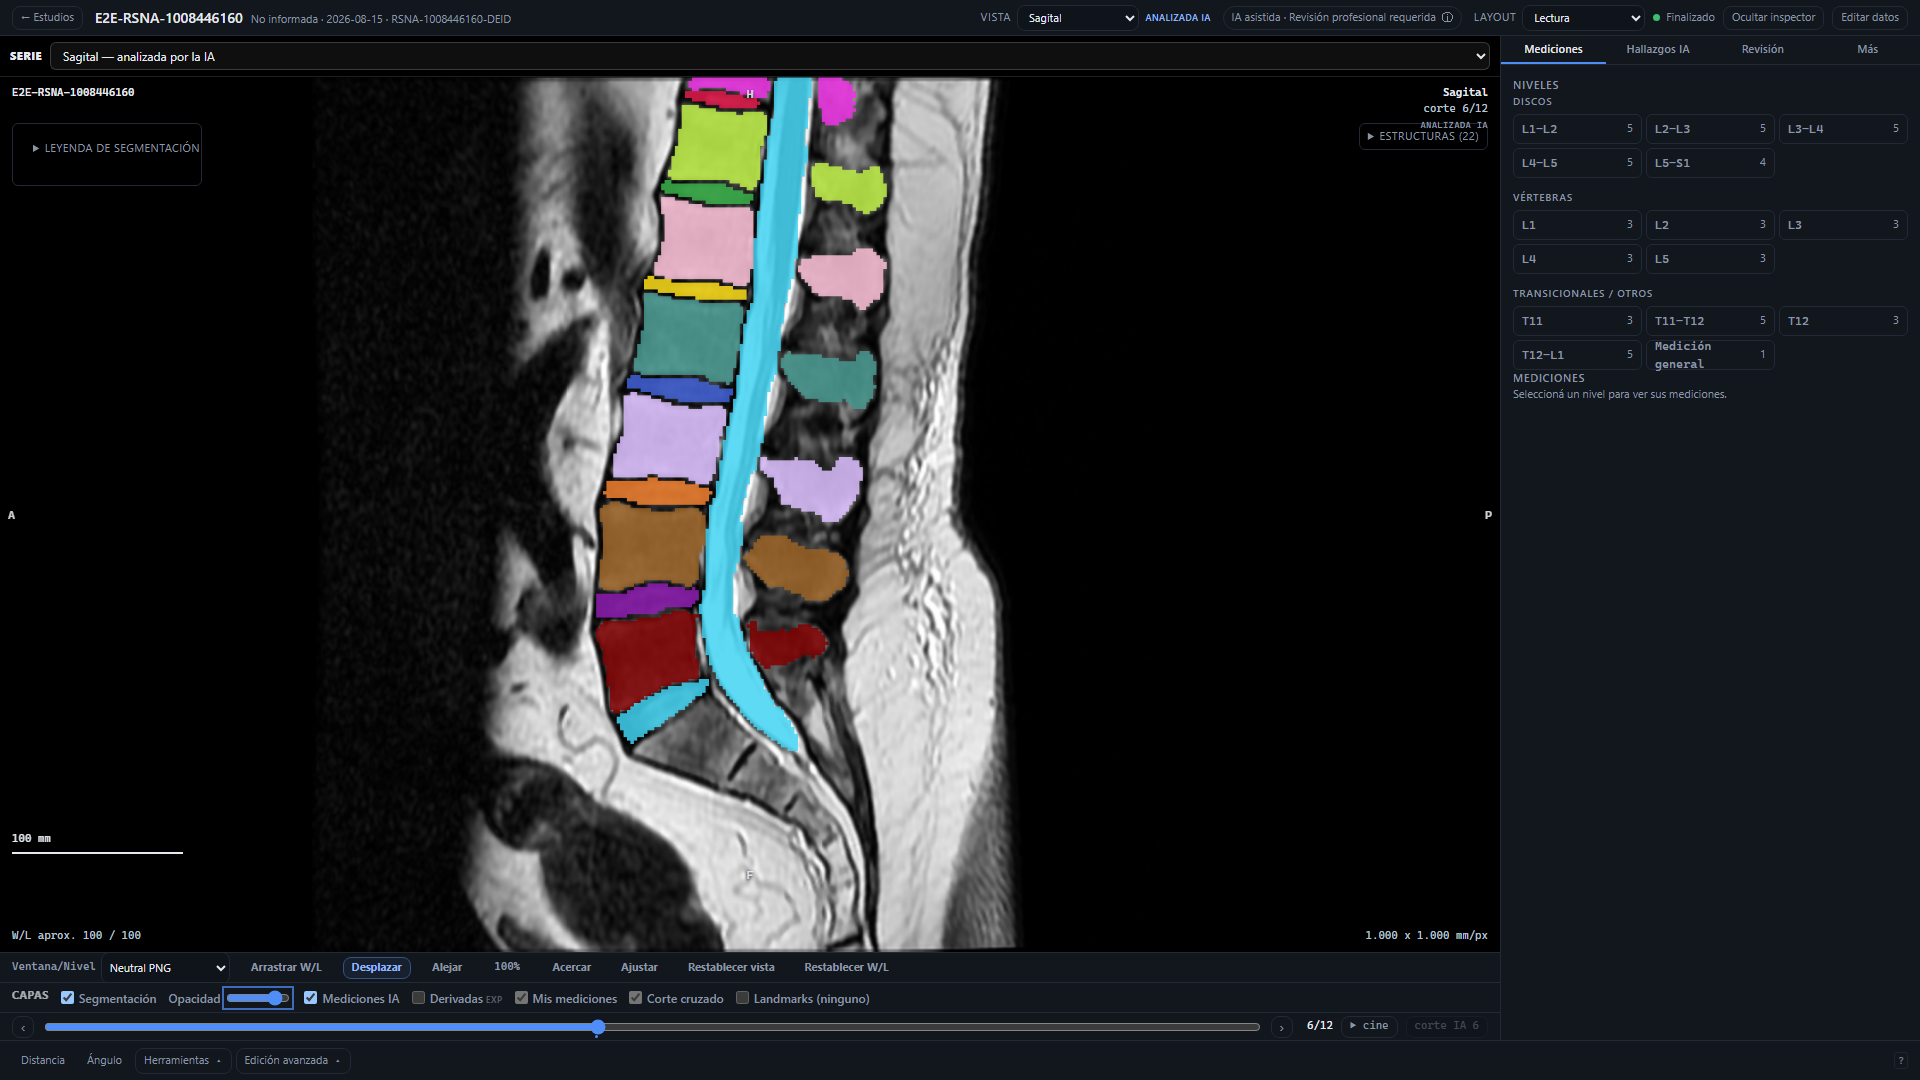
\includegraphics[width=\textwidth]{images/product_screenshots/fig_11_03_workspace_sagital.png}
\caption{Workspace sagital con la máscara superpuesta sobre la imagen original. Fuente: elaboración propia.}
\label{fig:cap11-workspace-sagital}
\end{figure}
Qué evidencia lo respalda. Coeficiente Dice macro de 0,893 sobre una partición retenida separada a nivel de paciente, con 152 pacientes de entrenamiento, 33 de validación y 33 de prueba. El artifact supera el umbral de calidad del proyecto y está registrado como baseline técnico validado. El protocolo completo, las particiones y el criterio del umbral se desarrollan en el Capítulo 13; la configuración de entrenamiento, en el Anexo E.

Qué límites tiene. El modelo produce clases agrupadas: no distingue una vértebra de otra ni un disco de otro. Toda afirmación sobre niveles anatómicos individuales depende del mecanismo descrito en la sección~\ref{sec:cap-asignacion-nivel-anatomico} y no del modelo. La evaluación mide coincidencia con las anotaciones del conjunto, de modo que reproduce también los criterios de quien anotó. No se informan métricas de distancia, que aportarían información sobre la precisión del contorno que el coeficiente Dice no captura en estructuras de tamaño considerable.

\section{Segmentación axial}

Qué hace. Delimita, sobre cortes axiales de los tres niveles discales inferiores, cuatro estructuras: disco intervertebral, elemento posterior, saco tecal y región anteroposterior.

Cómo funciona. Una red convolucional bidimensional entrenada sobre el conjunto de Sudirman y Al-Kafri. Las máscaras de referencia de ese conjunto no codifican las estructuras como índices consecutivos sino como valores de gris, de modo que el entrenamiento las remapea a seis clases conservando la nomenclatura de origen: las cuatro anatómicas y dos de fondo.

{\small
\setlength{\LTleft}{0pt}
\setlength{\LTright}{0pt}
\setlength{\tabcolsep}{3pt}
\renewcommand{\arraystretch}{1.18}
\begin{longtable}{>{\raggedright\arraybackslash}p{0.10\textwidth} >{\raggedright\arraybackslash}p{0.20\textwidth} >{\raggedright\arraybackslash}p{0.16\textwidth} >{\raggedright\arraybackslash}p{0.46\textwidth}}
\caption{Correspondencia entre clases del modelo axial y estructuras anatómicas.}\label{tab:cap-clases-modelo-axial}\\
\hline
\textbf{Índice} & \textbf{Clase} & \textbf{Valor de origen} & \textbf{Estructura anatómica} \\
\hline
\endfirsthead
\hline
\textbf{Índice} & \textbf{Clase} & \textbf{Valor de origen} & \textbf{Estructura anatómica} \\
\hline
\endhead
\hline
\endfoot
0 & background\_250 & 250 & Fondo del remapeo de entrenamiento \\
1 & raw\_0 & 0 & Fondo del conjunto de origen, correspondiente a la región que rodea al paciente \\
2 & raw\_50 & 50 & Disco intervertebral \\
3 & raw\_100 & 100 & Elemento posterior \\
4 & raw\_150 & 150 & Saco tecal \\
5 & raw\_200 & 200 & Región anteroposterior \\
\hline
\end{longtable}
}

La presencia de dos clases de fondo responde a que el remapeo de entrenamiento reserva el índice cero para su propio valor de fondo, mientras que el valor cero del conjunto de origen designa la región exterior al paciente. Ambas se excluyen de la representación visual. La nomenclatura de origen se conserva de forma deliberada, porque los nombres corresponden a valores de intensidad y no a términos clínicos: traducirlos a una terminología normalizada supondría atribuir una equivalencia que el conjunto de datos no declara.

La correspondencia queda congelada en el manifest del artifact y replicada en la configuración del runtime, con un validador que compara ambas fuentes. Renombrar una clase en el código invalida el manifest y deshabilita el modelo, restricción intencional para que el código y el artifact coincidan respecto de qué se entrenó.

\begin{figure}[htbp]
\centering
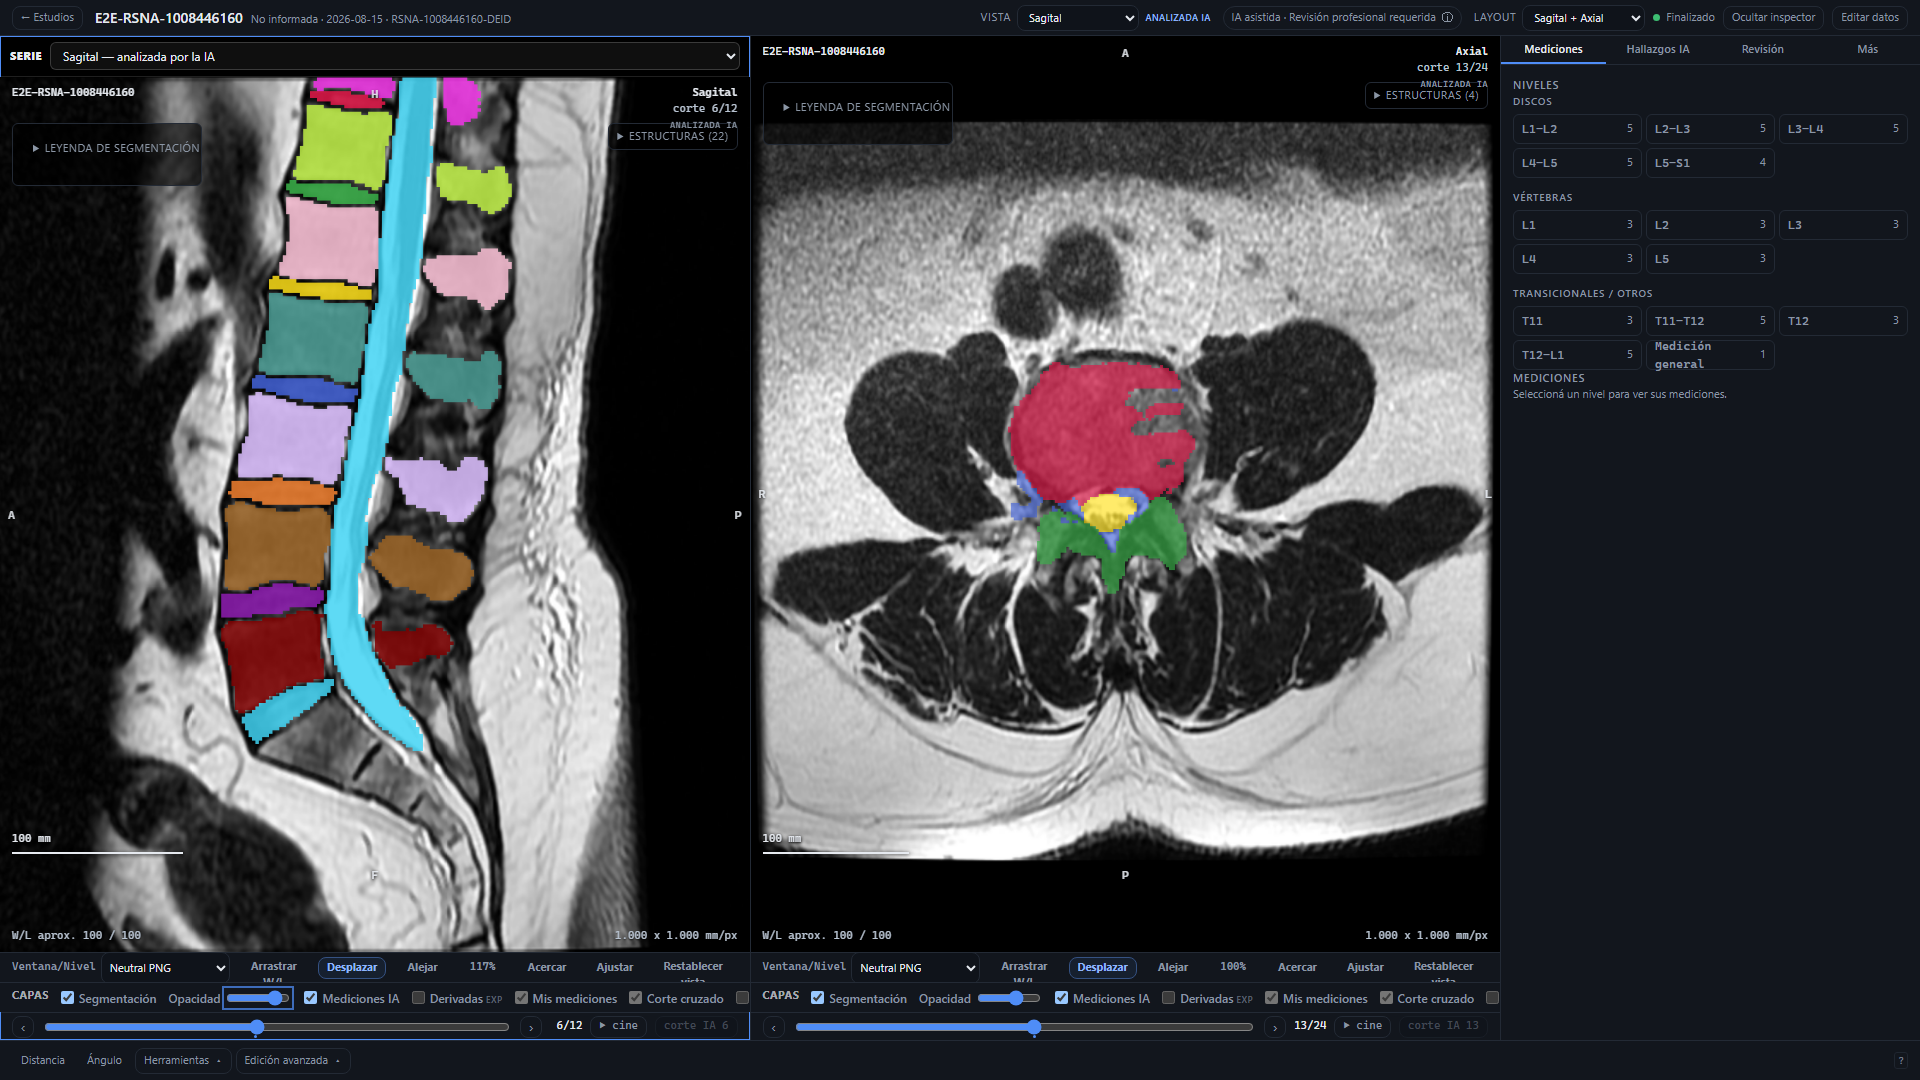
\includegraphics[width=\textwidth]{images/product_screenshots/fig_11_04_workspace_axial.png}
\caption{Workspace axial con la máscara superpuesta sobre la imagen original. Fuente: elaboración propia.}
\label{fig:cap11-workspace-axial}
\end{figure}
Qué evidencia lo respalda. Coeficiente Dice macro de 0,811 sobre las cuatro estructuras anatómicas y de 0,679 cuando se incluyen las dos clases de fondo, sobre una partición separada a nivel de paciente. La diferencia se explica porque una de las clases de fondo obtiene un coeficiente de 0,15 y arrastra el promedio.

% CROSS_REFERENCE_MAPPING_REQUIRED
Qué límites tiene. El artifact no alcanzó el umbral de calidad de 0,70 en la métrica que lo evalúa, que incluye las clases de fondo, y permanece registrado como candidato sin promoverse a baseline técnico. El umbral no se modificó para acomodar el resultado. La partición de prueba había sido evaluada previamente para una versión anterior del mismo modelo, de modo que el resultado es comparativo y no una validación sobre datos enteramente no observados. Los conteos de la partición de entrenamiento no fueron publicados en el manifest y su recuperación permanece pendiente. El capítulo 13 desarrolla estos tres puntos.

Corresponde además señalar que las anotaciones del conjunto de origen se realizaron sobre la ponderación T1 y la inferencia se ejecuta sobre T2, apoyándose en el co-registro nativo verificado entre ambas secuencias. Esa verificación se realizó sobre una muestra de los estudios y no sobre la totalidad del conjunto.

\section{Mediciones geométricas}

Qué hace. Deriva de las máscaras un conjunto acotado de magnitudes geométricas, cada una asociada a la estructura, el plano y el corte del que proviene.

Cómo funciona. Cada medición se emite con su valor, su unidad, el nivel anatómico cuando corresponde, el índice del corte, la confianza media del modelo sobre su propia máscara, el estado de revisión y el segmento de puntos del que se derivó el número. El valor automático y el valor corregido por el profesional se conservan en campos separados, de modo que una corrección no elimina el dato original. El conjunto de puntos viaja junto al valor y no se recalcula en la interfaz, para evitar que la representación gráfica y la tabla numérica discrepen.

{\scriptsize
\setlength{\LTleft}{0pt}
\setlength{\LTright}{0pt}
\setlength{\tabcolsep}{3pt}
\renewcommand{\arraystretch}{1.18}
\begin{longtable}{>{\raggedright\arraybackslash}p{0.19\textwidth} >{\raggedright\arraybackslash}p{0.22\textwidth} >{\raggedright\arraybackslash}p{0.29\textwidth} >{\raggedright\arraybackslash}p{0.10\textwidth} >{\raggedright\arraybackslash}p{0.12\textwidth}}
\caption{Catálogo de mediciones derivadas de las máscaras.}\label{tab:cap-mediciones-mascaras}\\
\hline
\textbf{Medición} & \textbf{Estructura} & \textbf{Método de cálculo} & \textbf{Unidad} & \textbf{Nivel} \\
\hline
\endfirsthead
\hline
\textbf{Medición} & \textbf{Estructura} & \textbf{Método de cálculo} & \textbf{Unidad} & \textbf{Nivel} \\
\hline
\endhead
\hline
\endfoot
Área, ancho y alto de disco & Disco intervertebral, una instancia por espacio discal & Área por recuento de píxeles convertido con el espaciado; ancho y alto sobre los ejes propios de la estructura & mm y mm² & Sí \\
Área, ancho y alto de cuerpo vertebral & Cuerpo vertebral, separado del arco posterior & Idéntico al anterior & mm y mm² & Sí \\
Área del canal & Canal completo visible en la serie & Recuento de píxeles convertido con el espaciado & mm² & No, corresponde al estudio \\
Diámetro anteroposterior del canal & Canal, acotado a la banda del disco correspondiente & Medición fila por fila dentro de la banda del nivel & mm & Sí \\
Ángulo segmentario & Dos cuerpos vertebrales contiguos & Ángulo entre los ejes de ancho de ambos cuerpos & Grados & Sí, con carácter experimental \\
Área, ancho y alto de estructuras axiales & Clases del módulo axial & Idéntico al de disco y cuerpo vertebral & mm y mm² & No \\
\hline
\end{longtable}
}

Tres decisiones de método requieren justificación explícita, y las tres surgieron de errores detectados durante el desarrollo.

Los ejes de medición son los de la estructura, no los de la imagen. El ancho y el alto se calculan sobre los ejes propios de cada estructura, obtenidos de los autovectores de la covarianza de la nube de píxeles y computados en milímetros para que un espaciado anisotrópico no incline los ejes por sí solo. La alternativa, una caja delimitadora alineada con la imagen, sobreestima toda estructura inclinada: en el espacio discal más angulado devolvía 25 milímetros de alto para un disco cuya dimensión habitual se sitúa entre 8 y 12. De los dos ejes resultantes, el más próximo a la horizontal se informa como ancho; ordenarlos por magnitud los intercambiaría en cualquier estructura más alta que ancha.

El área no requiere esa corrección, porque el recuento de píxeles no depende de la orientación.

El diámetro anteroposterior del canal se mide fila por fila. La primera implementación empleaba la caja delimitadora y devolvía 47 milímetros, valor incompatible con un canal lumbar: ese número correspondía al recorrido de la lordosis, dado que el centro del canal se desplaza alrededor de 35 milímetros entre los extremos de la serie. La medición fila por fila, acotada a la banda del disco, devuelve una componente conexa de 230 milímetros de extensión y entre 10 y 15 de ancho, con mediana de 13,1.

\begin{figure}[htbp]
\centering
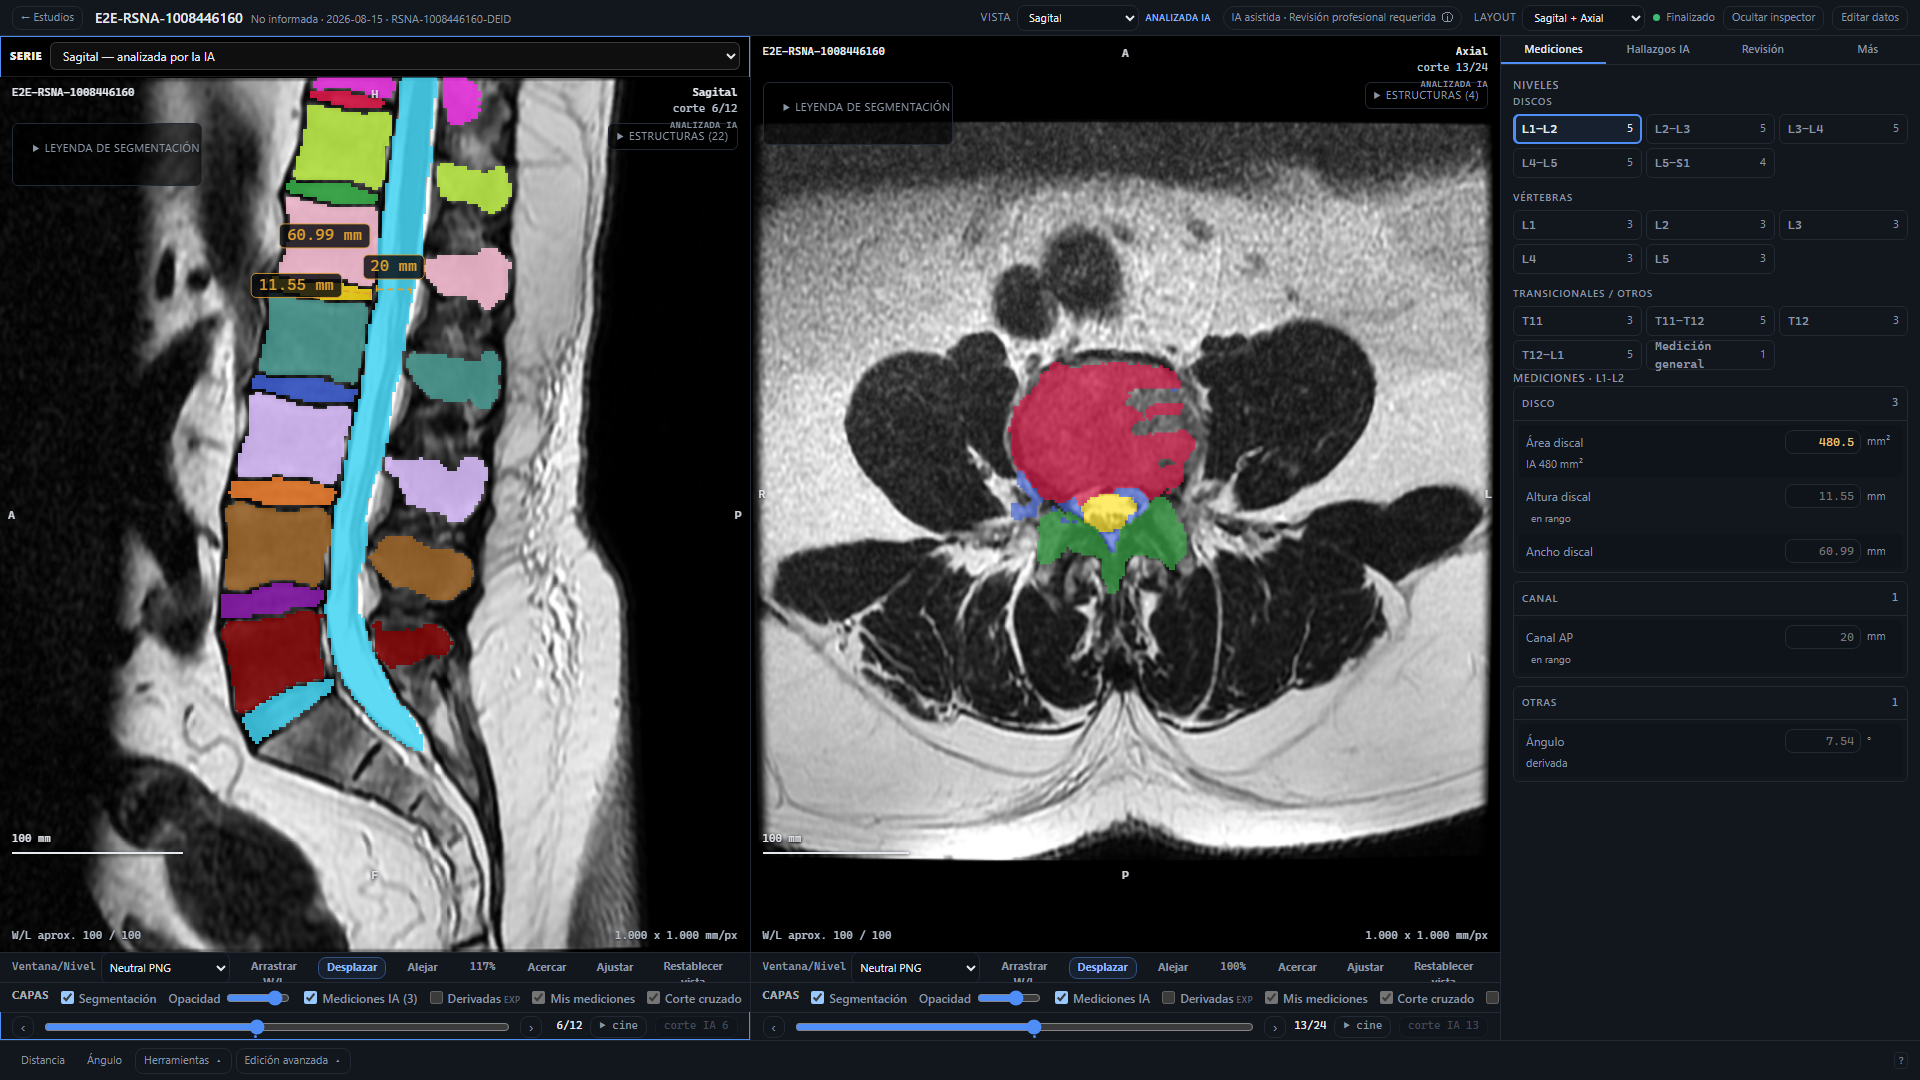
\includegraphics[width=\textwidth]{images/product_screenshots/fig_11_05_panel_mediciones.png}
\caption{Panel de mediciones con la estructura, el plano y el corte de origen de cada valor. Fuente: elaboración propia.}
\label{fig:cap11-panel-mediciones}
\end{figure}
Qué evidencia lo respalda. Una verificación por contraste contra rangos conocidos, desarrollada en el Capítulo 13. El diámetro anteroposterior del canal arroja una mediana compatible con el saco tecal lumbar, y la suma de ángulos segmentarios entre la primera y la quinta vértebra lumbar da 36 grados frente a una lordosis habitual de entre 40 y 60.

Qué límites tiene. Esa verificación no equivale a una validación. Un contraste con rangos poblacionales permite descartar valores manifiestamente incompatibles, pero no establece la exactitud de una medición individual. No existe comparación contra mediciones realizadas por profesionales sobre los mismos estudios, que requeriría un conjunto anotado específicamente para ese fin.

Dos límites adicionales se declaran de forma explícita. El primero es que el conjunto de datos denomina canal espinal a la clase segmentada sin precisar si delimita el canal óseo o su contenido dural, y el proyecto no atribuye una lectura que la fuente no declara. El segundo es que las mediciones son descriptores geométricos y no constituyen, por sí mismas, una clasificación clínica.

\section{Asignación de nivel anatómico}
\label{sec:cap-asignacion-nivel-anatomico}

Qué hace. Determina a qué espacio discal corresponde cada corte axial y cada medición, de modo que un valor pueda informarse como perteneciente a un nivel concreto y no de forma aislada.

Cómo funciona. Ninguna de las estructuras que el módulo axial segmenta es numerable por sí misma: para afirmar que una medición corresponde a un espacio discal determinado hay que contar espacios desde la unión lumbosacra, y un corte axial muestra uno solo. Antes de incorporar este mecanismo, la totalidad de las mediciones axiales se presentaba sin nivel asignado, lo que la interfaz mostraba como una falla cuando en realidad la ubicación nunca se había intentado.

El procedimiento resuelve la asignación en dos etapas, en coordenadas del paciente y no en índices de corte.

Sobre el plano sagital, por cada disco segmentado se publica su casco convexo expresado en coordenadas del paciente. La elección del casco convexo, en lugar de una caja delimitadora o de un centroide, responde a una propiedad del cálculo posterior: la pregunta que se formulará es entre qué dos valores queda comprendido el disco al proyectarlo sobre la normal del corte axial, y esa proyección es una función lineal, que sobre un conjunto acotado alcanza su mínimo y su máximo en un vértice del casco. El intervalo resultante es exacto para cualquier angulación, sin conservar la máscara completa. Una caja delimitadora produciría un intervalo mayor que el real, con lo que dos discos contiguos reclamarían el mismo corte; un centroide produciría uno menor, que es peor. La numeración se establece desde la unión lumbosacra hacia arriba.

Sobre el plano axial, para cada corte se calcula su normal a partir de los vectores de orientación registrados en la metadata y se proyecta sobre ella el casco convexo de cada disco. Si el desplazamiento del plano no queda comprendido entre los valores extremos de esa proyección, el disco no cruza ese corte. La resolución se realiza corte por corte y no una vez por serie, porque una serie axial lumbar habitualmente se adquiere en bloques angulados, uno por espacio discal: en el estudio de referencia empleado durante el desarrollo, los primeros cinco cortes presentan una angulación de 3,5 grados, los cinco siguientes de 5,9 y los últimos de 23. Propagar el nivel del corte analizado al resto de la serie situaría cerca de dos tercios de las mediciones bajo un nivel que no les corresponde.

Cuando un plano angulado cruza más de un espacio discal, se adjudica aquel al que atraviesa más cerca de su punto medio, que es el espacio sobre el cual la serie fue planificada, y la distancia se normaliza por la extensión del propio disco para que un espacio de mayor altura no resulte favorecido por su tamaño.

Qué evidencia lo respalda. El mecanismo está implementado y su salida expone el nivel de cada corte identificado por su índice, que el visor consume para presentar cada medición junto con su ubicación anatómica. No se dispone de una métrica de acierto de la asignación, es decir, de la proporción de cortes cuyo nivel se determina correctamente frente a una referencia. Es la principal evidencia faltante de esta capacidad y se declara como tal.

Qué límites tiene. Dos reglas de abstención acotan la capacidad de forma deliberada. Si el estudio muestra menos de cinco espacios discales, ninguna medición recibe nivel, antes que desplazar la numeración completa y adjudicar identificaciones incorrectas. Y si un corte no atraviesa ningún espacio discal, no se le asigna nivel: un corte axial puede haberse adquirido a la altura de un cuerpo vertebral, y adjudicarle el espacio más próximo situaría una medición bajo un nivel que no le corresponde, lo que resulta menos aceptable que no informarlo.

\section{Visualización y navegación por cortes}

Qué hace. Presenta la imagen original con la máscara superpuesta y permite recorrer la serie completa, conservando la relación entre cada resultado y el corte del que proviene.

Cómo funciona. El contrato volumétrico define, por serie, el plano, la cantidad de cortes, el corte de referencia, el eje de la secuencia, las dimensiones y el espaciado, junto con un catálogo en el que cada corte puede asociarse con una vista previa, un indicador de resultados y, cuando corresponda, superposición, puntos de referencia y mediciones. La responsabilidad se distribuye entre las tres capas: el módulo de inteligencia artificial genera una vista previa por corte y marca los que tienen resultado; el backend persiste el catálogo y publica los accesos autorizados, de modo que la navegación funciona con el módulo de inferencia apagado; el frontend presenta el recorrido con teclado o desplazamiento, indicador de corte actual y total, miniaturas, ajuste visual, control de opacidad y navegación desde una medición hacia su corte de origen.

\begin{figure}[htbp]
\centering
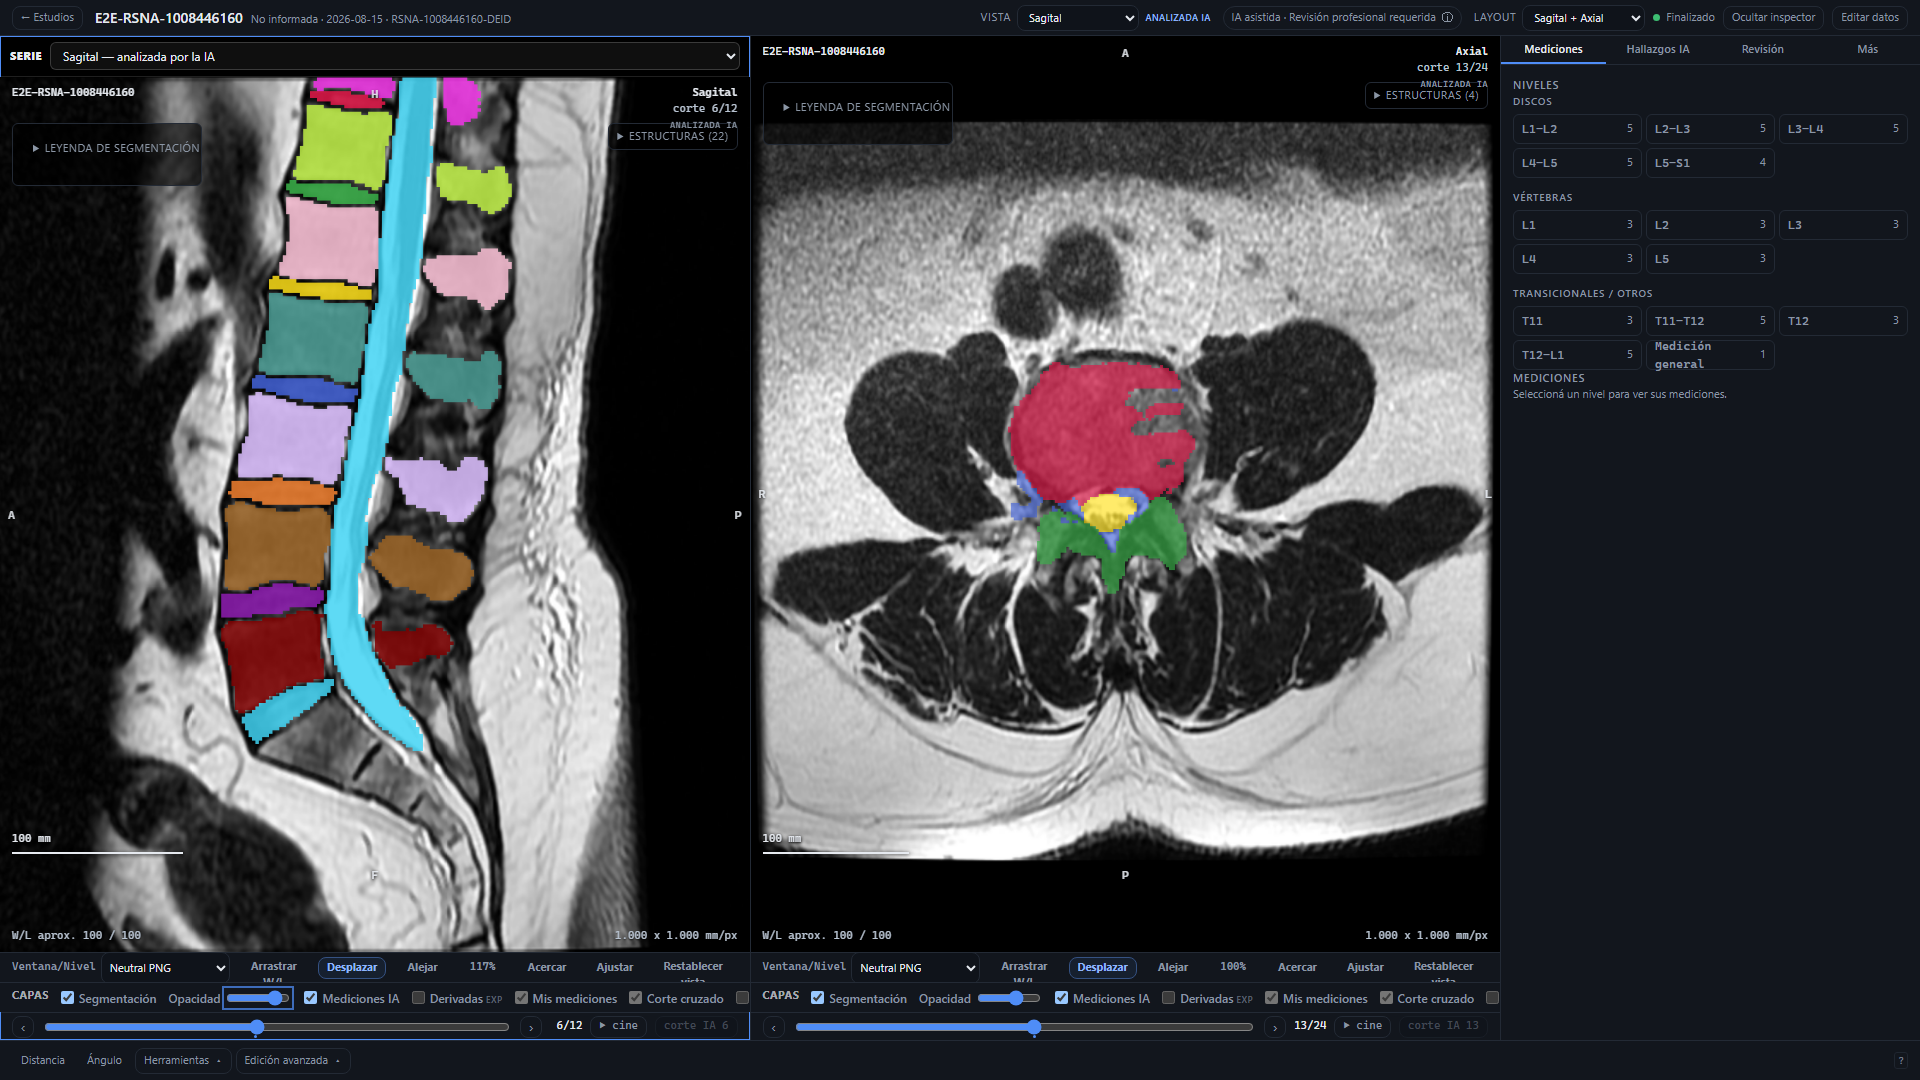
\includegraphics[width=\textwidth]{images/product_screenshots/fig_11_06_navegacion_full_series.png}
\caption{Navegación por cortes del volumen con el resultado vinculado a su corte. Fuente: elaboración propia.}
\label{fig:cap11-navegacion-full-series}
\end{figure}
Qué evidencia lo respalda. El procesamiento de la serie completa está implementado y los assets se persisten y se sirven por corte. Las pruebas verifican la cantidad y el orden de los cortes, el eje, el índice computacional y la numeración mostrada, con índice interno desde cero y numeración de interfaz desde uno.

Qué límites tiene. La superposición automática no se presupone para todos los cortes de todas las series: solo se muestra donde hay resultado, y los cortes sin inferencia lo declaran en lugar de presentarse vacíos. El visor no simula una correspondencia espacial entre el plano sagital y el axial cuando la metadata geométrica no permite demostrarla; la relación entre planos se establece por la asignación de nivel de la sección~\ref{sec:cap-asignacion-nivel-anatomico} y no por una superposición supuesta. La integración definitiva de los contratos congelados en el frontend y el cierre del recorrido extremo a extremo con interfaz permanecen pendientes.

\section{Revisión profesional y salida editable}

Qué hace. Permite que el profesional acepte, observe, corrija o descarte cada resultado, y reúne las estructuras, las mediciones y las observaciones en una salida editable que incluye un preinforme automático revisable.

Cómo funciona. La revisión no es una etapa posterior sino parte del flujo: los controles se ubican junto al resultado que califican, y cada decisión queda registrada con su autor y su estado. El valor automático y el corregido se conservan por separado, de modo que la corrección no borra la evidencia original.

El preinforme se construye mediante plantillas que combinan los valores derivados de las máscaras con formulaciones fijas asociadas a cada estructura, nivel y medición. No proviene de un modelo de lenguaje ni de una inferencia clínica, sino de una transformación determinística de datos geométricos ya calculados y visibles. Esa distinción importa: dado un mismo conjunto de máscaras y mediciones, produce siempre el mismo texto, y cada afirmación puede rastrearse hasta la estructura y el corte que la originan.

\begin{figure}[htbp]
\centering
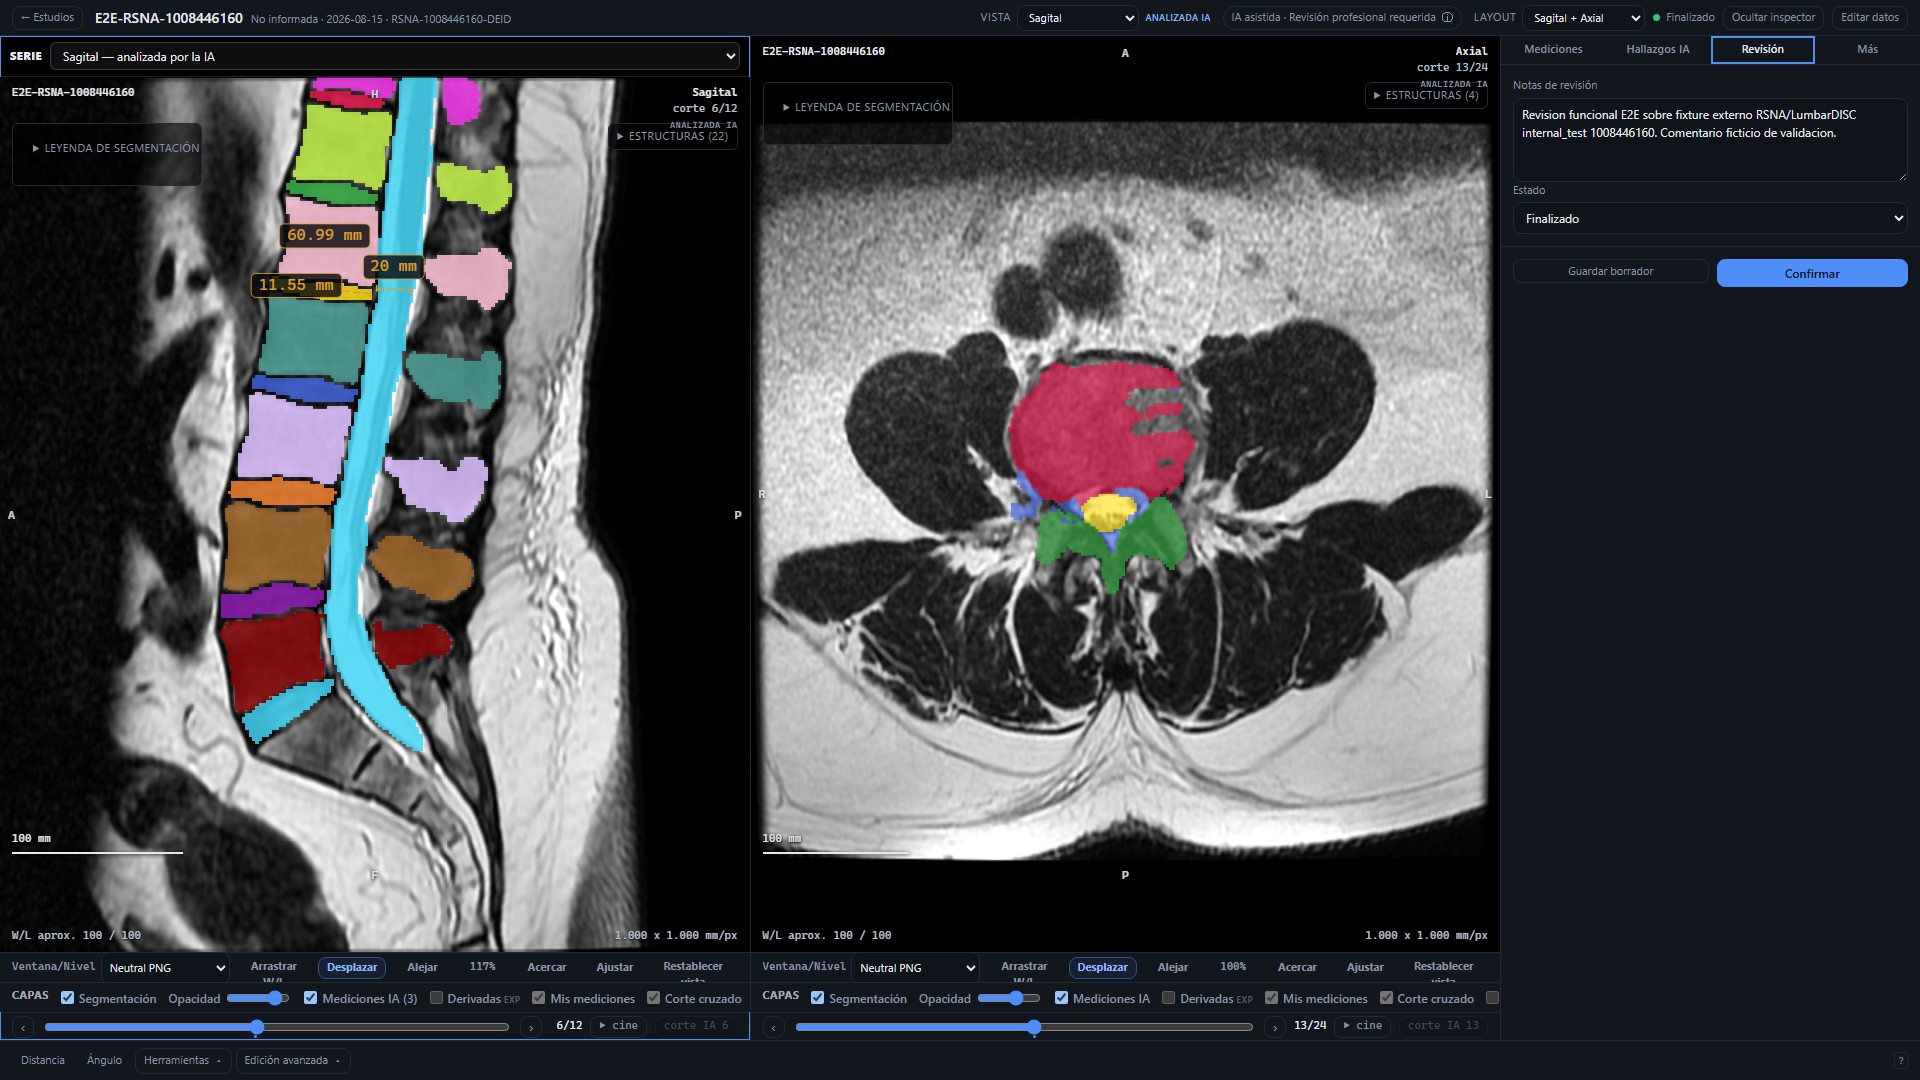
\includegraphics[width=\textwidth]{images/product_screenshots/fig_11_07_revision_profesional.png}
\caption{Controles de revisión profesional sobre una estructura segmentada. Fuente: elaboración propia.}
\label{fig:cap11-revision-profesional}
\end{figure}

\begin{figure}[htbp]
\centering
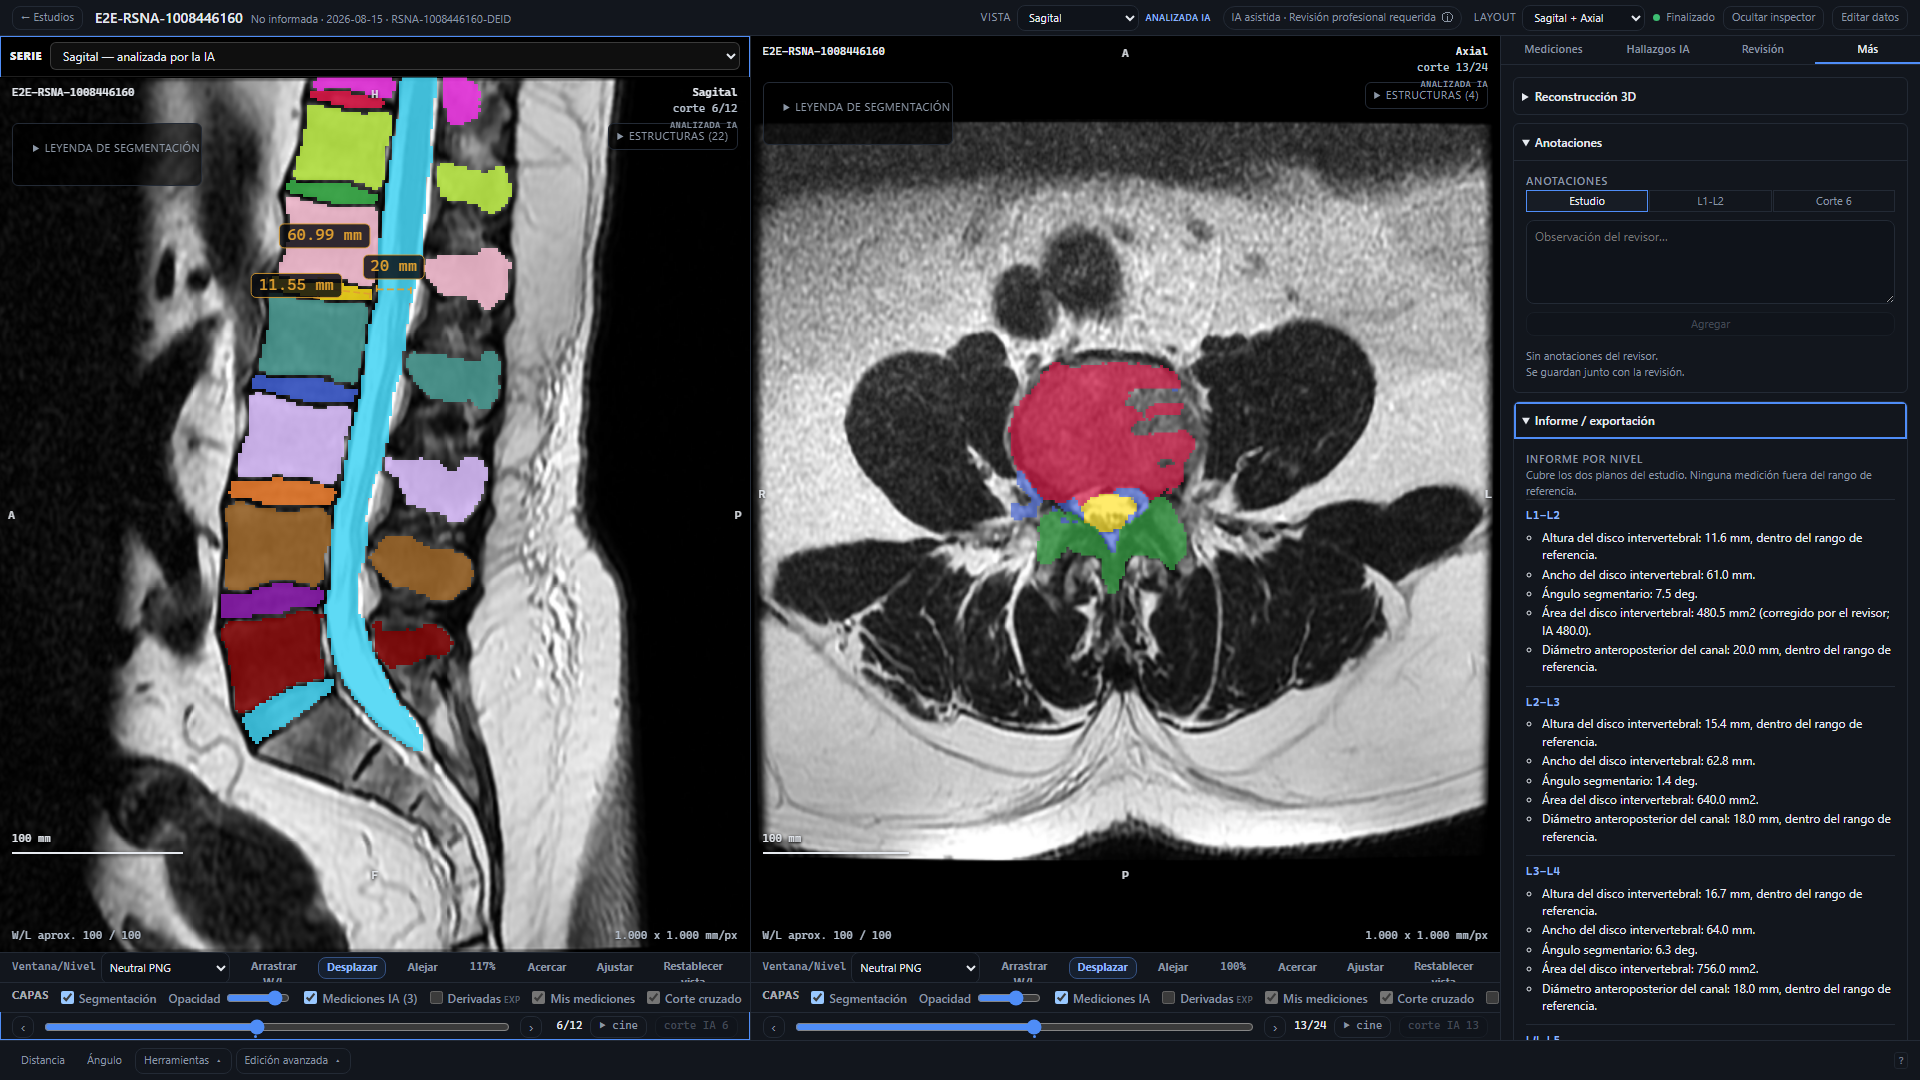
\includegraphics[width=\textwidth]{images/product_screenshots/fig_11_08_preinforme_revisable.png}
\caption{Preinforme automático revisable con estructuras, mediciones y estado de revisión. Fuente: elaboración propia.}
\label{fig:cap11-preinforme-revisable}
\end{figure}
Qué evidencia lo respalda. El flujo de revisión está implementado y persistido, y la reapertura de un estudio recupera el estado de revisión junto con los resultados. El relevamiento con profesionales identificó la posibilidad de corregir manualmente cada resultado como el requisito más votado para confiar en una segmentación automática, según se informa en la sección 8.12.

Qué límites tiene. El preinforme es un punto de partida editable y no un informe clínico: su función es reducir la transcripción manual de valores y organizarlos en un orden anatómico previsible, mientras la redacción final, la interpretación y la responsabilidad permanecen en el profesional. La evaluación de utilidad del flujo de revisión con profesionales sobre el producto integrado permanece pendiente.

\section{Persistencia, reapertura y trazabilidad}

Qué hace. Conserva cada corrida con su modelo, su artifact, sus resultados, sus mediciones y su estado de revisión, de modo que un estudio pueda recuperarse más tarde sin volver a ejecutar la inferencia.

Cómo funciona. Un estudio actúa como contenedor lógico y una corrida representa una ejecución concreta, de manera que ejecutar de nuevo no sobrescribe la evidencia anterior. Los estudios de un mismo paciente se vinculan mediante una referencia de sujeto seudonimizada, sin exponer datos identificatorios en el flujo de trabajo. Cada corrida genera identificadores que permiten seguirla: el del caso, el de la ejecución, el que agrupa ambos planos y el que correlaciona solicitudes y registros técnicos.

\begin{figure}[htbp]
\centering
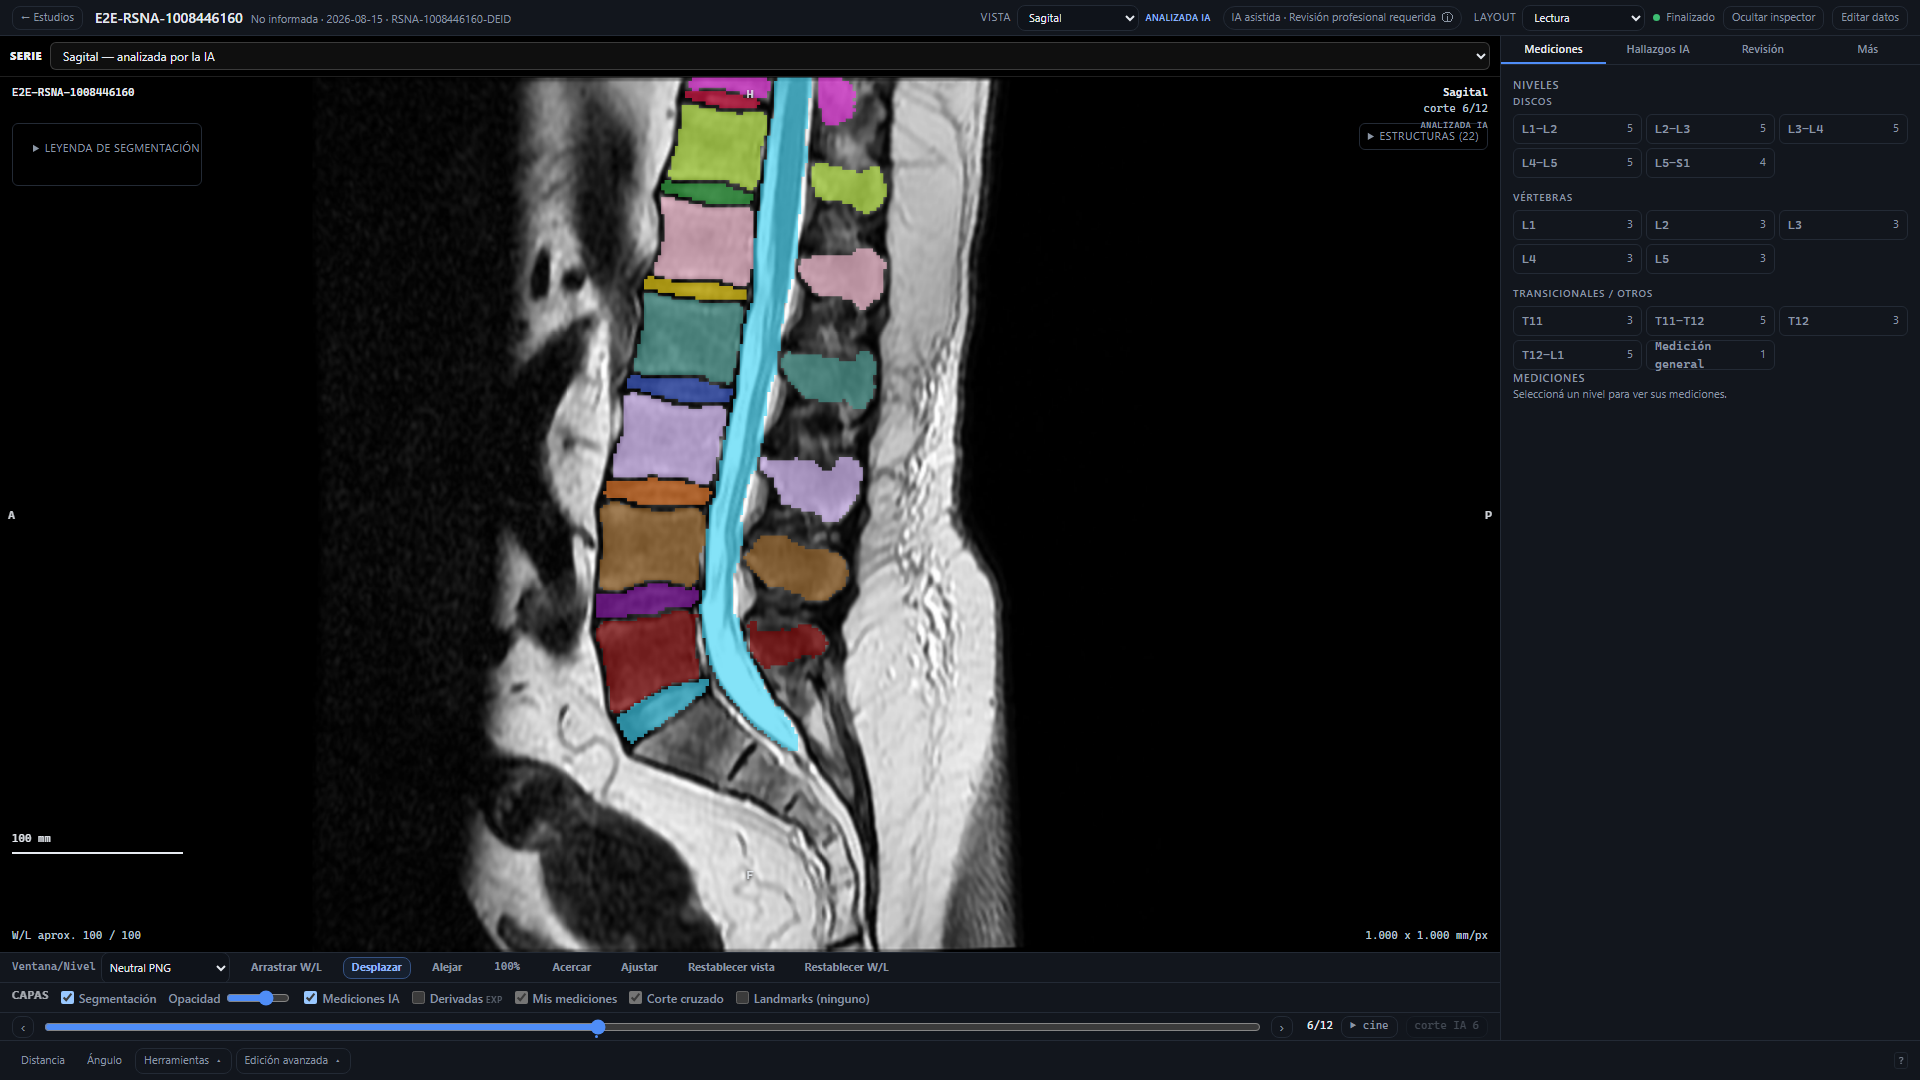
\includegraphics[width=\textwidth]{images/product_screenshots/fig_11_09_persistencia_nueva_sesion.png}
\caption{Historial de corridas y reapertura de un estudio ya procesado. Fuente: elaboración propia.}
\label{fig:cap11-persistencia-nueva-sesion}
\end{figure}
Qué evidencia lo respalda. La prueba de aceptación de esta capacidad consiste en abrir un estudio persistido con el módulo de inferencia apagado y comprobar que recupera resultados, mediciones y estado de revisión. Esa prueba está incorporada al repositorio y se ejecuta como regresión.

Qué límites tiene. Las corridas anteriores a la incorporación del catálogo de cortes conservan únicamente los assets que existían en su momento y se abren en modo de compatibilidad, sin fabricar un catálogo que no se generó.

\section{Seguridad y estados degradados}

Qué hace. Restringe las operaciones según el rol del usuario y comunica de forma explícita cuándo un componente no está disponible, en lugar de presentar la indisponibilidad como un resultado del análisis.

Cómo funciona. Las operaciones protegidas requieren autenticación y autorización, las cuentas nuevas permanecen pendientes de aprobación, los assets no se sirven mediante rutas internas y los secretos se mantienen fuera del código. El frontend no se comunica directamente con el módulo de inferencia: todas las operaciones pasan por el backend, lo que permite aplicar autorización y conservar el resultado aunque el servicio de inferencia esté caído.

El sistema distingue el modo de ejecución solicitado del modo efectivamente aplicado. Una corrida solo se informa como inferencia real cuando existieron un artifact identificable, un manifest coherente, una arquitectura compatible, una entrada procesable y una ejecución exitosa. Si alguna de esas condiciones falta, la respuesta declara el estado degradado y no se registra como resultado válido.

\begin{figure}[htbp]
\centering
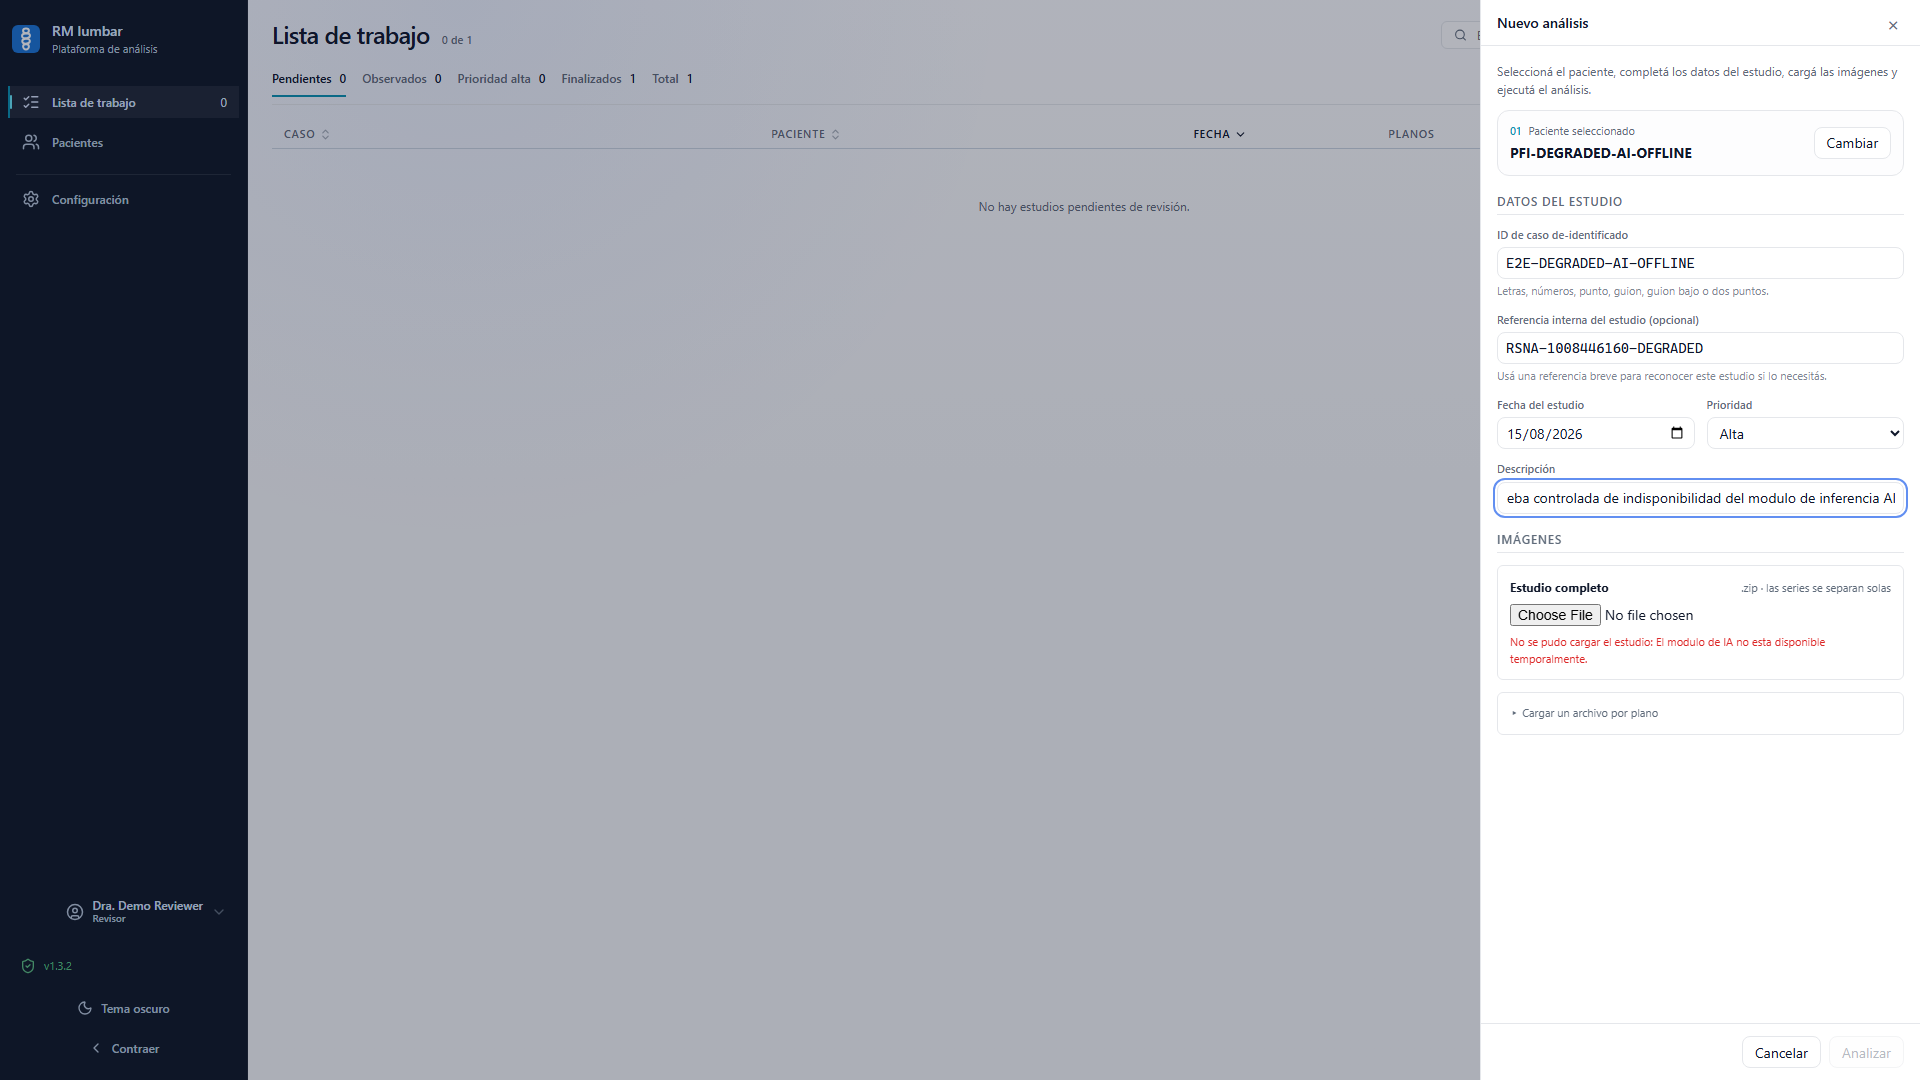
\includegraphics[width=\textwidth]{images/product_screenshots/fig_11_10_estado_degradado_ai_no_disponible.png}
\caption{Estado degradado informado de forma explícita ante indisponibilidad del módulo de inferencia. Fuente: elaboración propia.}
\label{fig:cap11-estado-degradado-ai}
\end{figure}
Qué evidencia lo respalda. Pruebas de autenticación, autorización, contratos, auditoría y comportamiento ante archivo inválido, artifact ausente, rol insuficiente y asset faltante. El contrato público no expone probabilidades, salidas crudas, mapas de confianza ni rutas internas.

Qué límites tiene. El endurecimiento de la configuración de seguridad para un entorno productivo permanece como evolución posterior. Las medidas descritas corresponden a un prototipo académico y no constituyen una evaluación formal de cumplimiento normativo.

\section{Capacidades desarrolladas y no expuestas}

Dos líneas de trabajo produjeron modelos entrenados y congelados que no forman parte de las capacidades del producto. Se documentan aquí porque constituyen trabajo realizado y porque su exclusión es una decisión de alcance que conviene justificar, no una omisión.

\subsection{Estimación de hallazgos estructurales por nivel}

Se entrenó y congeló un modelo multitarea que, a partir de las series sagitales, produce ocho estimaciones estructurales por nivel discal: grado de degeneración discal, cambio de señal de platillo, cambios de platillo vertebral superior e inferior, desplazamiento vertebral, hernia, reducción de altura y protrusión.

El modelo se entrenó sobre 992 muestras y se seleccionó sobre 248 de validación. La evaluación final se realizó una única vez sobre una partición sellada de 278 niveles discales correspondientes a 39 pacientes, sin solapamiento de pacientes con el conjunto de desarrollo y sin inspeccionarla durante la selección del modelo. El grado de degeneración y el cambio de señal de platillo son tareas multiclase, de cinco y cuatro categorías respectivamente, y se evalúan mediante F1 macro y exactitud balanceada; las seis restantes son binarias y se evalúan mediante F1, área bajo la curva ROC y precisión promedio.

{\scriptsize
\setlength{\LTleft}{0pt}
\setlength{\LTright}{0pt}
\setlength{\tabcolsep}{3pt}
\renewcommand{\arraystretch}{1.18}
\begin{longtable}{>{\raggedright\arraybackslash}p{0.23\textwidth} >{\raggedright\arraybackslash}p{0.12\textwidth} >{\raggedright\arraybackslash}p{0.08\textwidth} >{\raggedright\arraybackslash}p{0.15\textwidth} >{\raggedright\arraybackslash}p{0.11\textwidth} >{\raggedright\arraybackslash}p{0.16\textwidth} >{\raggedright\arraybackslash}p{0.09\textwidth}}
\caption{Desempeño de la estimación estructural sobre la partición sellada.}\label{tab:cap-desempeno-estimacion-estructural}\\
\hline
\textbf{Estimación} & \textbf{Tipo} & \textbf{F1} & \textbf{Exactitud balanceada} & \textbf{ROC-AUC} & \textbf{Precisión promedio} & \textbf{Línea base} \\
\hline
\endfirsthead
\hline
\textbf{Estimación} & \textbf{Tipo} & \textbf{F1} & \textbf{Exactitud balanceada} & \textbf{ROC-AUC} & \textbf{Precisión promedio} & \textbf{Línea base} \\
\hline
\endhead
\hline
\endfoot
Protrusión discal & Binaria & 0,846 & — & 0,899 & 0,903 & — \\
Reducción de altura discal & Binaria & 0,733 & — & 0,890 & 0,823 & — \\
Cambio de platillo inferior & Binaria & 0,751 & — & 0,787 & 0,794 & — \\
Cambio de platillo superior & Binaria & 0,730 & — & 0,771 & 0,770 & — \\
Grado de degeneración discal & 5 clases & 0,492 & 0,521 & — & — & 0,200 \\
Cambio de señal de platillo & 4 clases & 0,315 & 0,422 & — & — & 0,250 \\
Hernia discal & Binaria & 0,189 & — & 0,669 & 0,085 & 0,036 \\
Desplazamiento vertebral & Binaria & 0,125 & — & 0,788 & 0,089 & 0,032 \\
\hline
\end{longtable}
}

La línea base indica el valor que alcanzaría un clasificador aleatorio: en las tareas multiclase corresponde al azar uniforme y en las binarias a la prevalencia de la clase positiva, que es la referencia adecuada para la precisión promedio cuando las clases están desbalanceadas.

El desempeño es marcadamente heterogéneo y las ocho estimaciones no admiten la misma lectura. La protrusión y la reducción de altura alcanzan valores consistentes en las tres métricas. Los cambios de platillo se sitúan en un rango intermedio. Las dos tareas multiclase superan con claridad el azar uniforme, en 32 y 17 puntos porcentuales respectivamente, pero permanecen lejos de un valor utilizable en un flujo asistido.

Las dos últimas requieren una lectura más cuidadosa. El desplazamiento vertebral aparece en 9 de las 278 muestras y la hernia en 10, es decir, con prevalencias en torno al 3 \%. Con ese desbalance, su precisión promedio de 0,089 y 0,085 equivale a 2,75 y 2,36 veces la línea base, de modo que no es correcto describirlas como indistinguibles del azar. El área bajo la curva del desplazamiento vertebral, de 0,788, indica además una capacidad de ordenamiento razonable. Sin embargo, sus F1 de 0,125 y 0,189 muestran que, con el umbral operativo empleado, la clasificación positiva sigue siendo débil: el modelo ordena mejor de lo que decide.

Esa heterogeneidad está registrada en el propio contrato del sistema. El desplazamiento vertebral y la hernia se encuentran marcados como no soportados para producto, de modo que la distinción entre estimaciones utilizables y no utilizables no es una lectura posterior del documento sino una propiedad del artifact congelado.

% CROSS_REFERENCE_MAPPING_REQUIRED
Ninguna de las ocho estimaciones se expone en el producto. La razón no es únicamente el desempeño de las tareas más débiles, sino que el prototipo no dispone de un mecanismo para comunicar al profesional que dos estimaciones presentadas con la misma jerarquía visual difieren en confiabilidad en un orden de magnitud. Exponer probabilidades queda excluido por diseño, y presentar las ocho como equivalentes induciría a confiar por igual en resultados que no lo son. La decisión responde al mismo criterio que la sección 13.7 desarrolla con otro caso: una salida se publica cuando puede verificarse y comunicarse junto con su incertidumbre, no cuando puede calcularse.

El entrenamiento continúa sobre un conjunto de datos de mayor tamaño, de modo que las cifras informadas corresponden al estado congelado en esta instancia y no al desempeño final de la línea. Su promoción a capacidad del producto requeriría, como mínimo, ampliar el conjunto en las tareas de baja prevalencia y resolver cómo comunicar la diferencia de confiabilidad entre estimaciones.

\subsection{Clasificación de estenosis subarticular}

Se entrenó y evaluó internamente un modelo de estenosis subarticular sobre cortes axiales, empleando el conjunto RSNA y LumbarDISC, y su checkpoint fue congelado. La capacidad permanece bloqueada porque el clasificador requiere como entrada una región de interés anatómica que el sistema no genera de forma automática: el modelo axial disponible no incluye una clase de vértebra, de modo que no existe una referencia anatómica desde la cual derivar esa región. Los sustitutos evaluados se descartaron por razones metodológicas.

Se trata de un bloqueo de capacidad y no de un trabajo pendiente de ejecución. Su resolución depende de una etapa de localización anatómica que no está disponible.

\section{Estado consolidado de las capacidades}

{\scriptsize
\setlength{\LTleft}{0pt}
\setlength{\LTright}{0pt}
\setlength{\tabcolsep}{3pt}
\renewcommand{\arraystretch}{1.18}
\begin{longtable}{>{\raggedright\arraybackslash}p{0.35\textwidth} >{\raggedright\arraybackslash}p{0.12\textwidth} >{\raggedright\arraybackslash}p{0.45\textwidth}}
\caption{Estado de las capacidades al cierre de esta entrega.}\label{tab:cap-estado-capacidades}\\
\hline
\textbf{Capacidad} & \textbf{Sección} & \textbf{Estado} \\
\hline
\endfirsthead
\hline
\textbf{Capacidad} & \textbf{Sección} & \textbf{Estado} \\
\hline
\endhead
\hline
\endfoot
Ingesta DICOM con identificación de series & 11.2 & Implementada \\
Preparación y corrección geométrica & 11.2 & Implementada \\
Segmentación sagital & 11.3 & Implementada y evaluada; baseline técnico \\
Segmentación axial & 11.4 & Implementada y evaluada; artifact por debajo del umbral \\
Mediciones geométricas & 11.5 & Implementadas y persistidas; verificadas por contraste, sin validación \\
Asignación de nivel anatómico & 11.6 & Implementada; sin métrica de acierto \\
Visualización y navegación por cortes & 11.7 & Implementada; integración final en el frontend pendiente \\
Revisión profesional & 11.8 & Implementada en su flujo principal \\
Preinforme automático revisable & 11.8 & Implementado; editable y no diagnóstico \\
Persistencia, reapertura y trazabilidad & 11.9 & Implementadas \\
Seguridad, roles y estados degradados & 11.10 & Implementados; endurecimiento productivo posterior \\
Estimación de hallazgos estructurales & 11.11.1 & Desarrollada y evaluada sobre partición sellada; no expuesta por desempeño heterogéneo \\
Clasificación de estenosis subarticular & 11.11.2 & Bloqueada \\
Recorrido extremo a extremo con interfaz & — & Pendiente \\
Validación profesional sobre el producto & — & Pendiente \\
Comparación longitudinal & — & Futura \\
Despliegue en la plataforma objetivo & — & Planificado \\
\hline
\end{longtable}
}

Esta tabla describe el estado del producto y no sustituye el backlog técnico. Una capacidad solo se declara implementada cuando existe en el flujo, cuenta con pruebas y su evidencia puede localizarse. Las tres capacidades cuya evidencia visual todavía no se incorporó al documento se identifican mediante los espacios reservados de las figuras correspondientes.
